%%%%%%%%%%%%%%%%%%%%%%%%%%%%%%%%%%%%%%%%%%%%%%
\section{Beam plug}
\label{sec:beamplug}
\fixme{Rearrange the text so beam plug is described here. The beam window penetration through the cryostat insulation layers is described in the crystat section}
The main function of the beam window system is to allow charged particles from the H4 beam line to enter the TPC with minimal energy loss and multiple scattering. The system penetrates through the cryostat insulation layers, displaces approximately 45cm of passive LAr layer, and extends inside the active TPC region through an opening in the TPC field cage. To keep the primary stainless-steel membrane of the cryostat intact, the beam window is divided into two independent subsystems. The first system (system 1) is installed inside the cryostat insulation layer and ends at the primary cryostat membrane. The second system (system 2) is inside the LAr portion of the cryostat. For NP04, the H4 beam line is designed to be able to inject beam into the LAr cryostat at three different locations. Due to various engineering and safety constraints, only one of the beam injection points will have the full beam window system installed. The sketch of the beam window system is shown in Figure~\ref{fig:beamwindow_fig1}. The details of the design are described in the following sections.
\begin{cdrfigure}[Beam window systems]{beamwindow_fig1}{Beam window system 1 and 2.}
  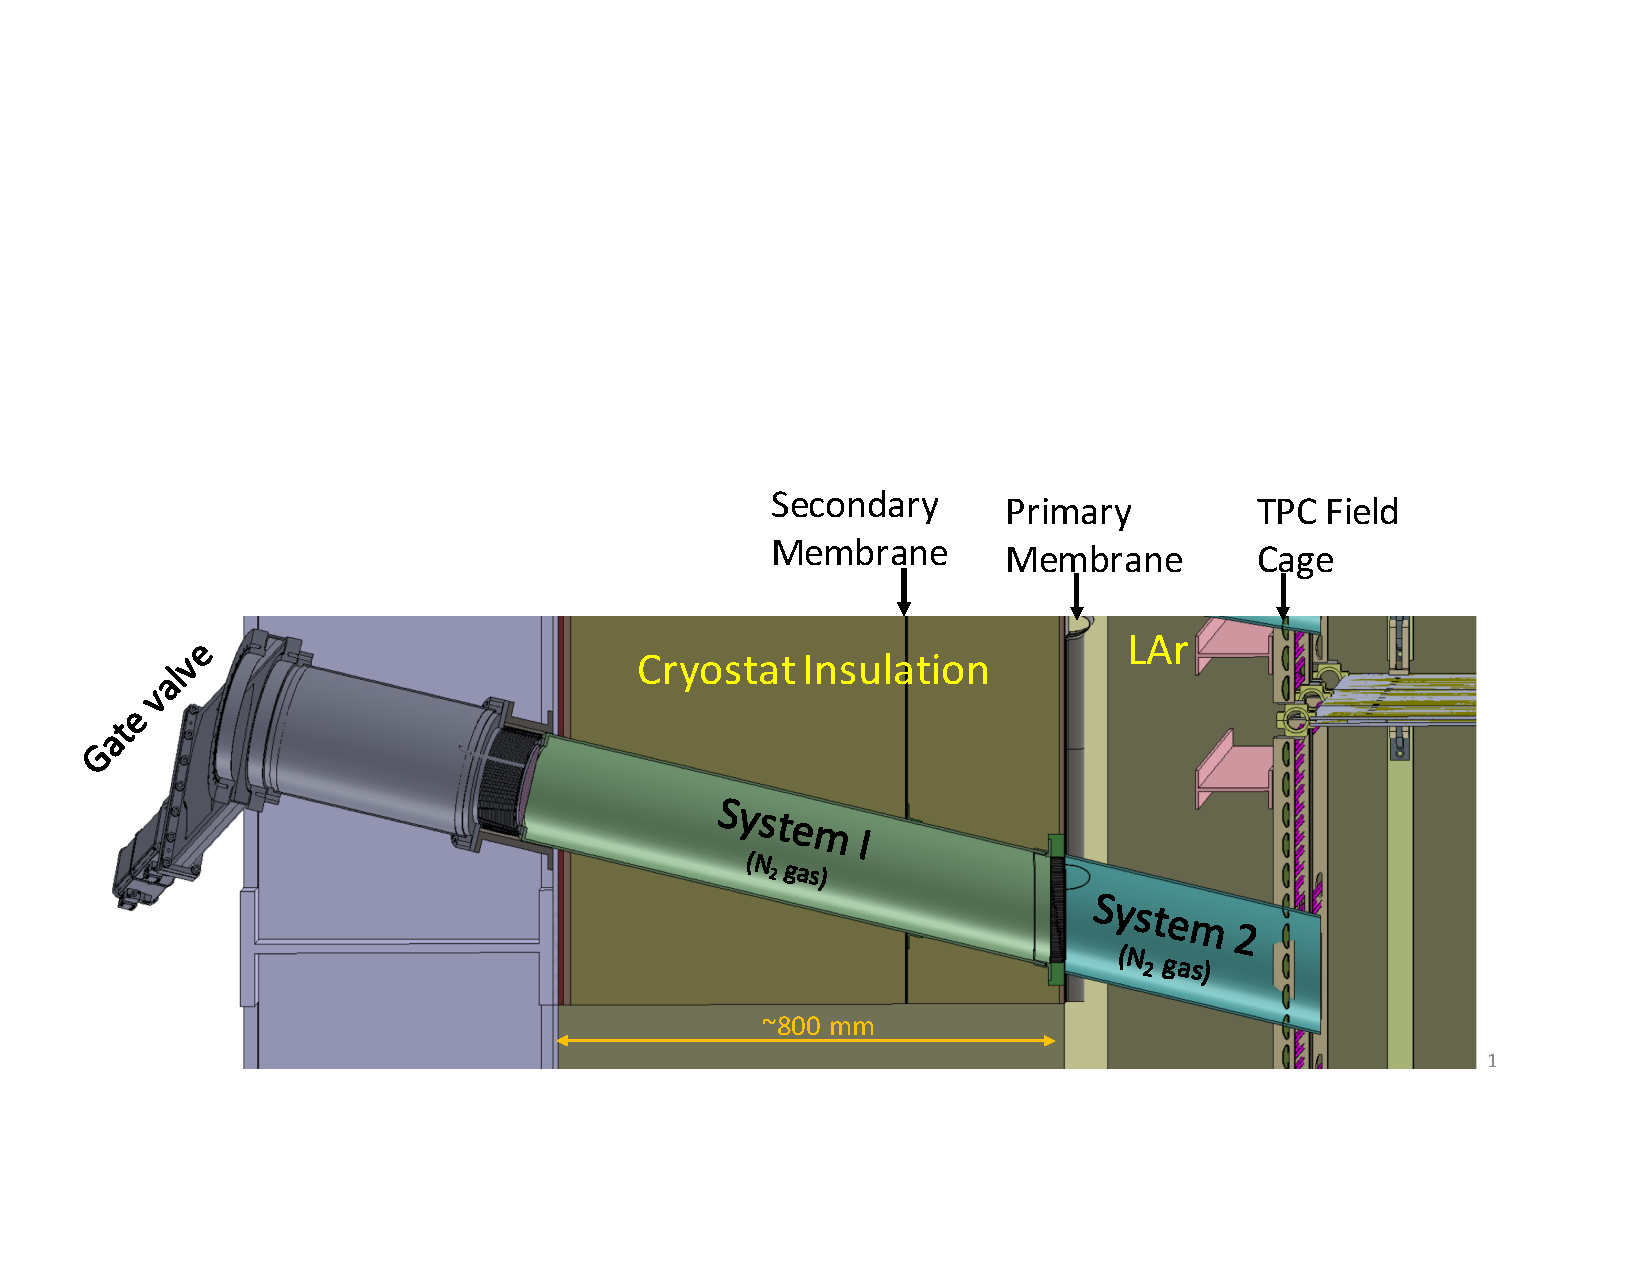
\includegraphics[width=0.90\textwidth]{beamwindow_system1and2.pdf}
\end{cdrfigure}

\subsection{System 1}
A close-up view of the System 1 beam window is shown in Figure~\ref{fig:beamwindow_zoom}. The system 1 beam window is a cylindrical G10 (OD$\approx$22cm) tube with a nomex honeycomb core at each end. The tube is filled with dry nitrogen gas and maintained at about 1 atm of pressure. It is designed to provide thermal insulation with a heat load of less than 5W/$m^2$. As shown in Figure~\ref{fig:beamwindow_fig1}, system 1 beam window extends to the external steel support structure of the cryostat. The other end of the beam window is in physical contact with the cryostat's primary membrane. When the cryostat is filled with LAr, the nomex honeycomb core provides the structural support to prevent the membrane from bulging outward. The honeycomb core on the other end of the tube, where the bellow is located, provides thermal insulation to keep ice from building up on the outer surface. The secondary membrane will be bonded onto a cylindrical disk attached to the G10 shell during installation. The system 1 beam window is anchored to the outer steel structure of the cryostat with a flange. As an additional safety measure, there is an option to install a gate valve on the external end of the beam window.
\begin{cdrfigure}[Beam window 1 zoomed]{beamwindow_zoom}{A detailed view of system 1 beam widnow.}
  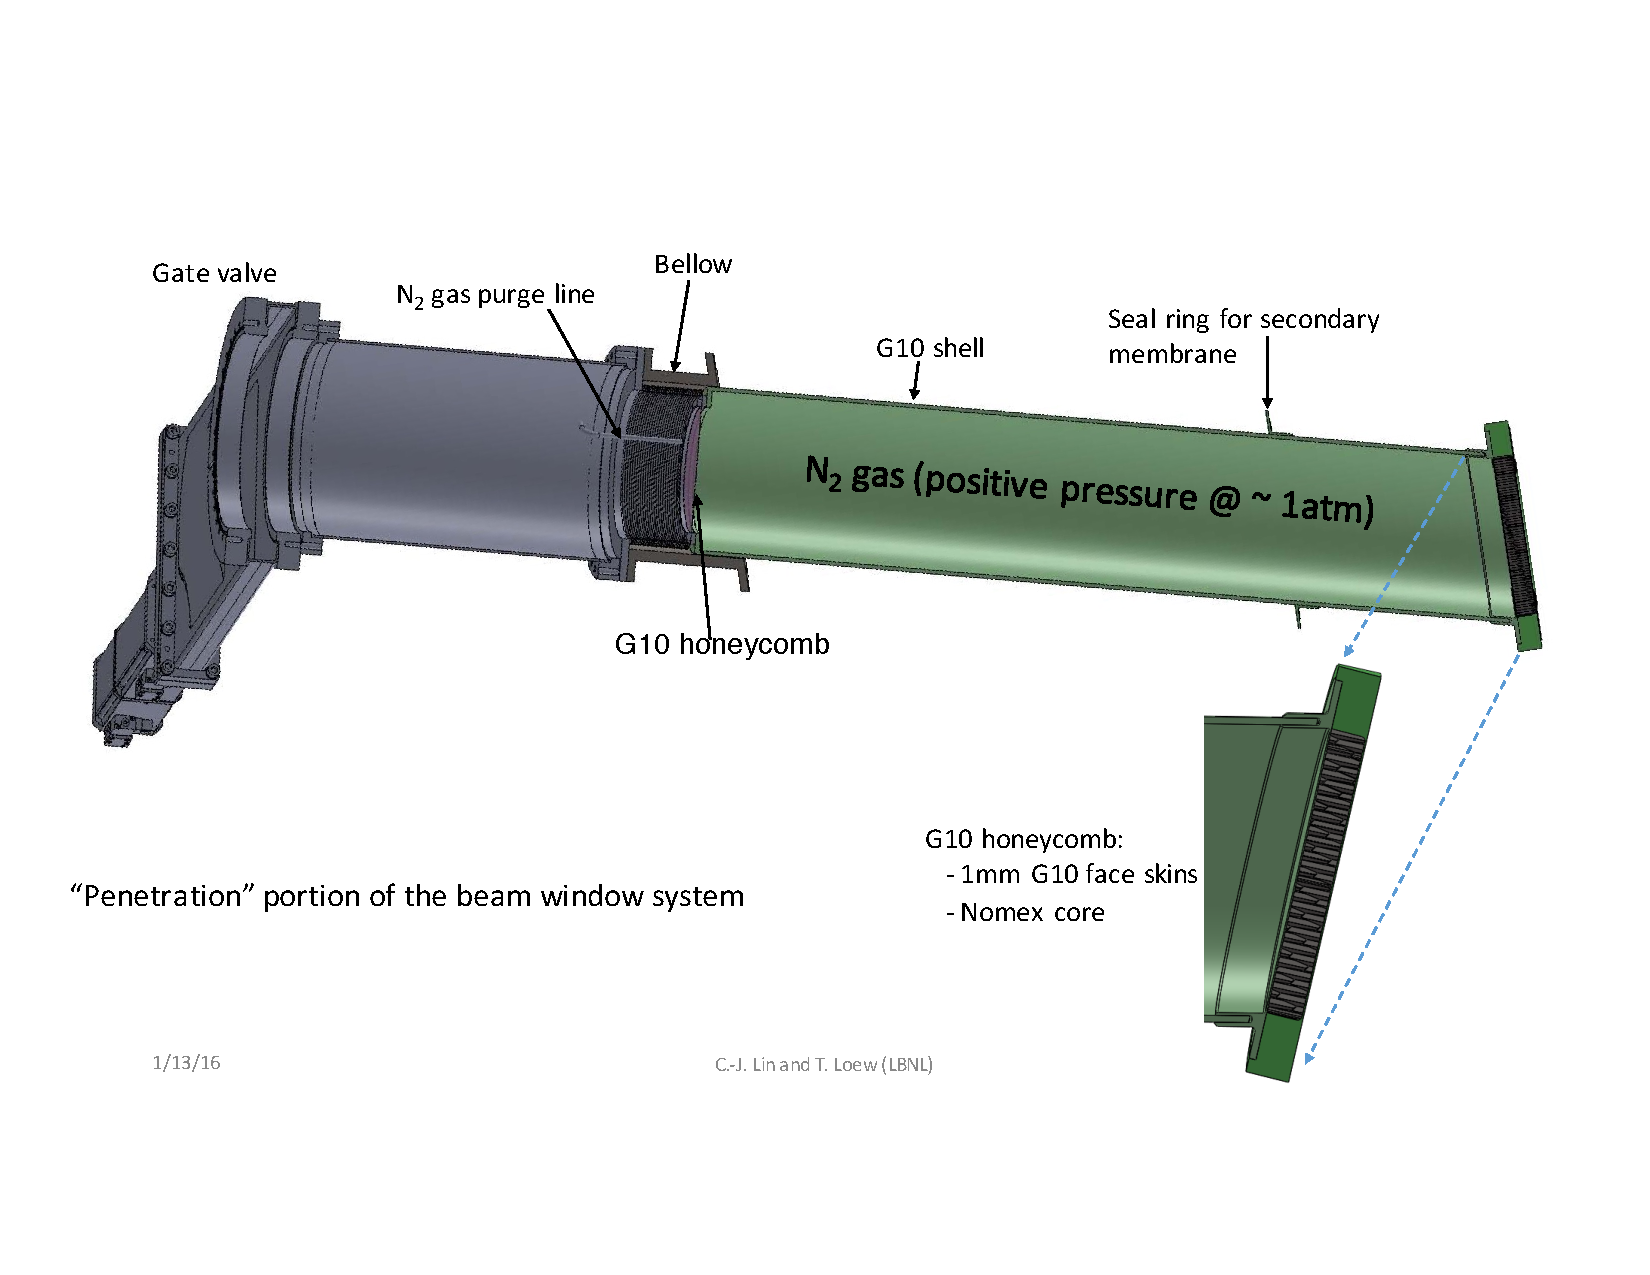
\includegraphics[width=0.90\textwidth]{beamwindow_system1zoom.pdf}
\end{cdrfigure}


\subsection{System 2 (``beam plug'')}
The system 2 beam window (a.k.a. beam plug) is designed to displace the passive LAr layer between the TPC field cage and the inner crystat membrane. As illustrated in Figure~\ref{fig:beamwindow_fig2}, it is a cylidrical glass-fiber composite (type-V) pressure vessel about 50cm in length and  22cm in diameter. It is filled with dry nitrogen gas to about 3 atm at room temperature. The beam plug is secured to the field cage support structure (see Figure~\ref{fig:beamwindow_fig3}). The field cage support is designed with sufficient strength to withstand the expected buoyancy force of about 200N when the beam plug is immersed in LAr. 

At nominal operation, the voltage difference across the beam plug could be as high as 160kV. To minimize electrical discharges, the beam plug is divided into sections and each section is bonded to a stainless-steel conductive grading rings. The grading rings are conected in series with two parallel path of resistor chains. There are 7 grading rings. The ring that is closest to the field cage is electrically connected to one of the aluminum field cage profiles. The last ring near the cryostat wall is grounded to the stainless steel membrane. The type and value of the resistor is still under evaluation. A likely candidate is the high voltage Super Mox 5GOhm resistor by OHMITE. The maximum total power dissipated by the resistor chain is about 2W.

\begin{cdrfigure}[System 2 beam window]{beamwindow_fig2}{System 2 beam window. It is a type-V all composite pressure vessel filled with dry nitrogen gas to about 3 atm at room temperature. The vessel is about 50cm in length and about 22cm in diameter. The pressure vessel is divided into sections with each section bonded to a stainless-steel grading ring. The grading rings are connected by two parallel paths of resistor chain.}
  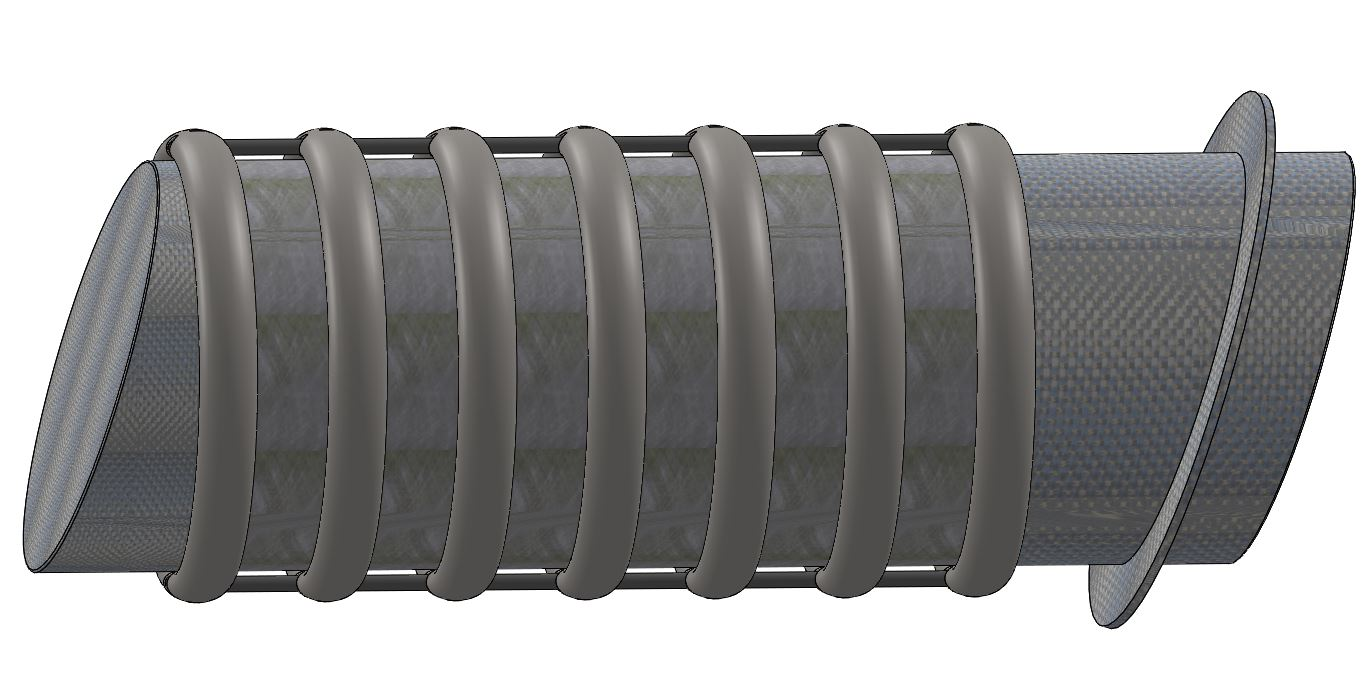
\includegraphics[width=0.7\textwidth]{beamwindow_system2.jpg}
\end{cdrfigure}

\begin{cdrfigure}[System 2 beam window mounting scheme]{beamwindow_fig3}{System 2 beam window mounting scheme (preliminary). The beam plug is mounted to the field cage support structure.}
  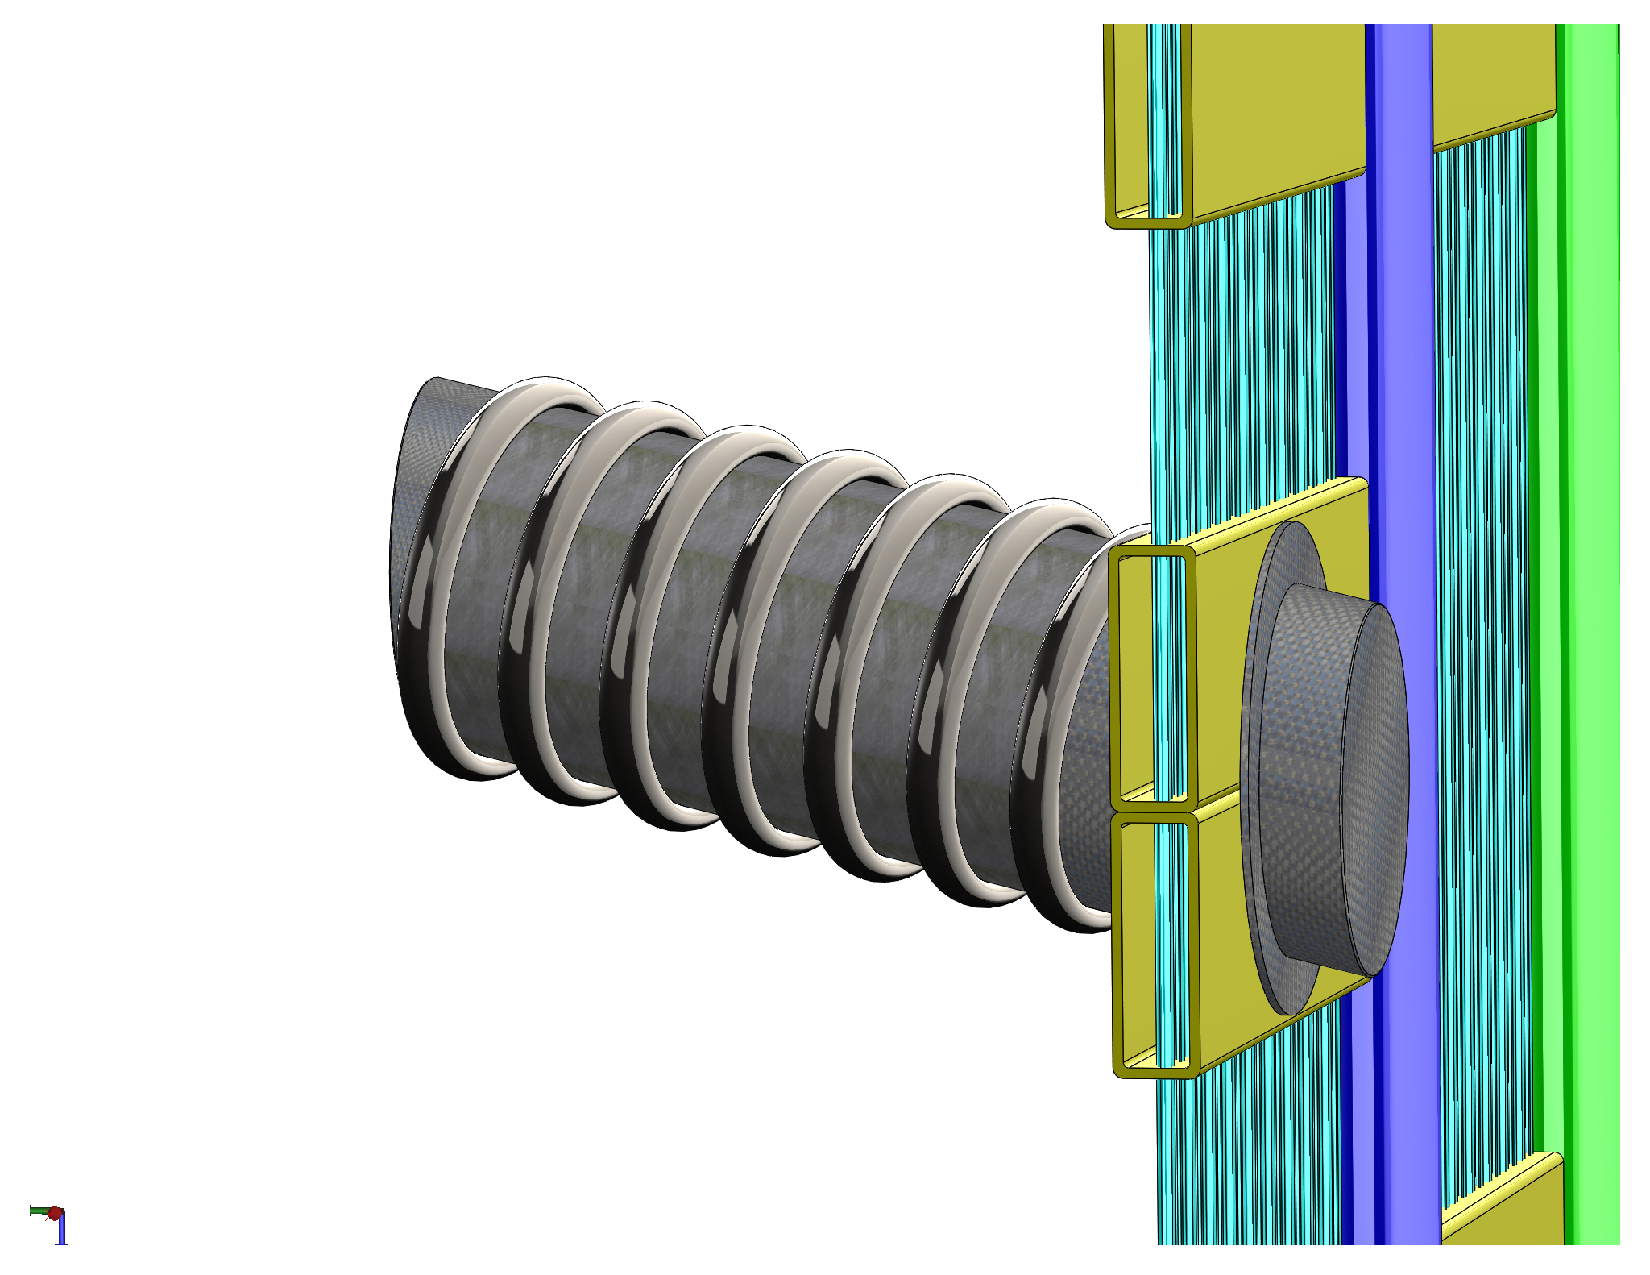
\includegraphics[width=0.7\textwidth,height=0.3\textheight]{beamwindow_system2_mount.pdf}
\end{cdrfigure}

\subsection{Beam window system tests} 

\subsubsection{System 1 Tests}
Discuss system 1 beam window test at LBNL.

\subsubsection{System 2 Tests}

\subsubsubsection{BLANCHE Test-stand}
Discuss HV test of system 2 beam window in BLANCHE test-stand

\subsubsubsection{SLAC beam test}
Discuss SLAC beam test.
\begin{cdrfigure}[SLAC beam test]{beamwindow_SLAC}{Test setup for the SLAC beam test.}
  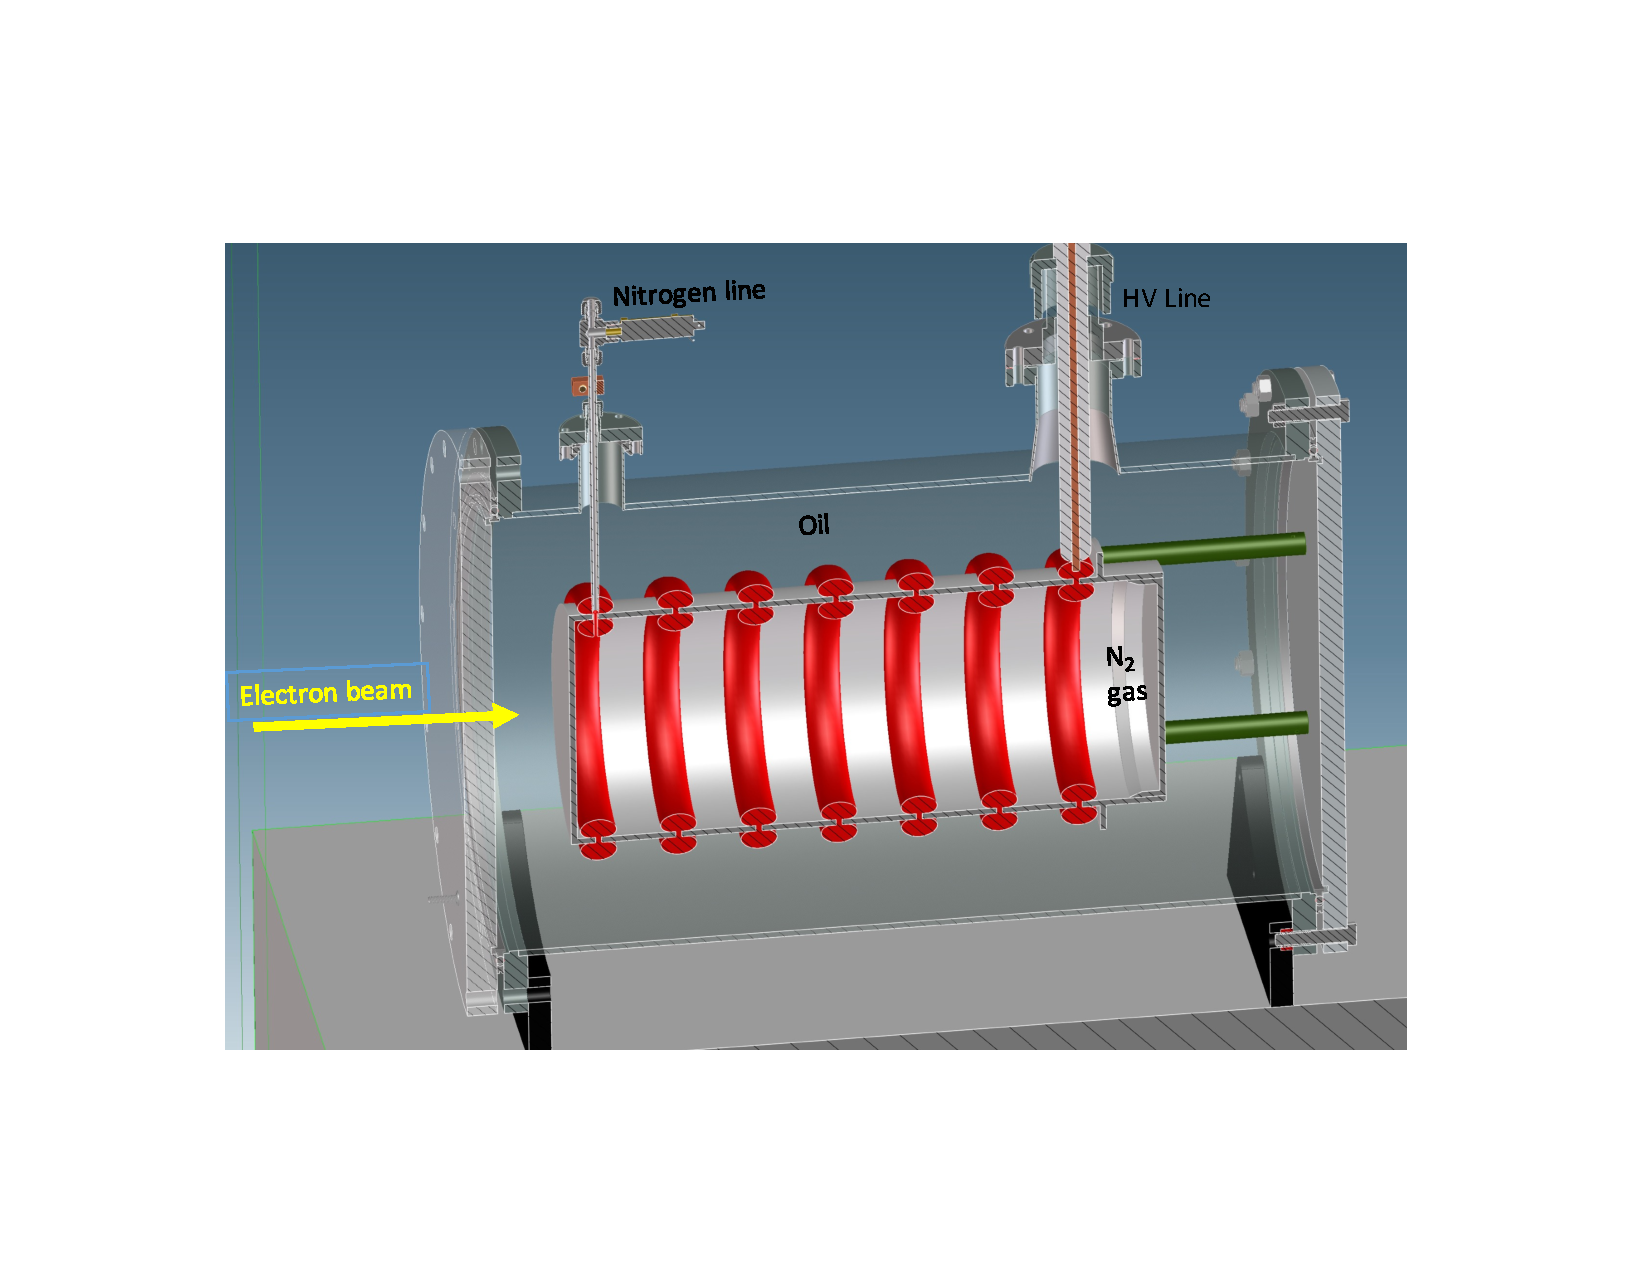
\includegraphics[width=0.8\textwidth]{beamwindow_SLACtest.pdf}
\end{cdrfigure}

\subsubsubsection{Full integration test in 35-ton cryostat}
Discuss field cage mock-up test.
\begin{cdrfigure}[SLAC beam test]{beamwindow_PC4}{Field cage mock-up high voltage test in 35-ton (preliminary drawing).}
  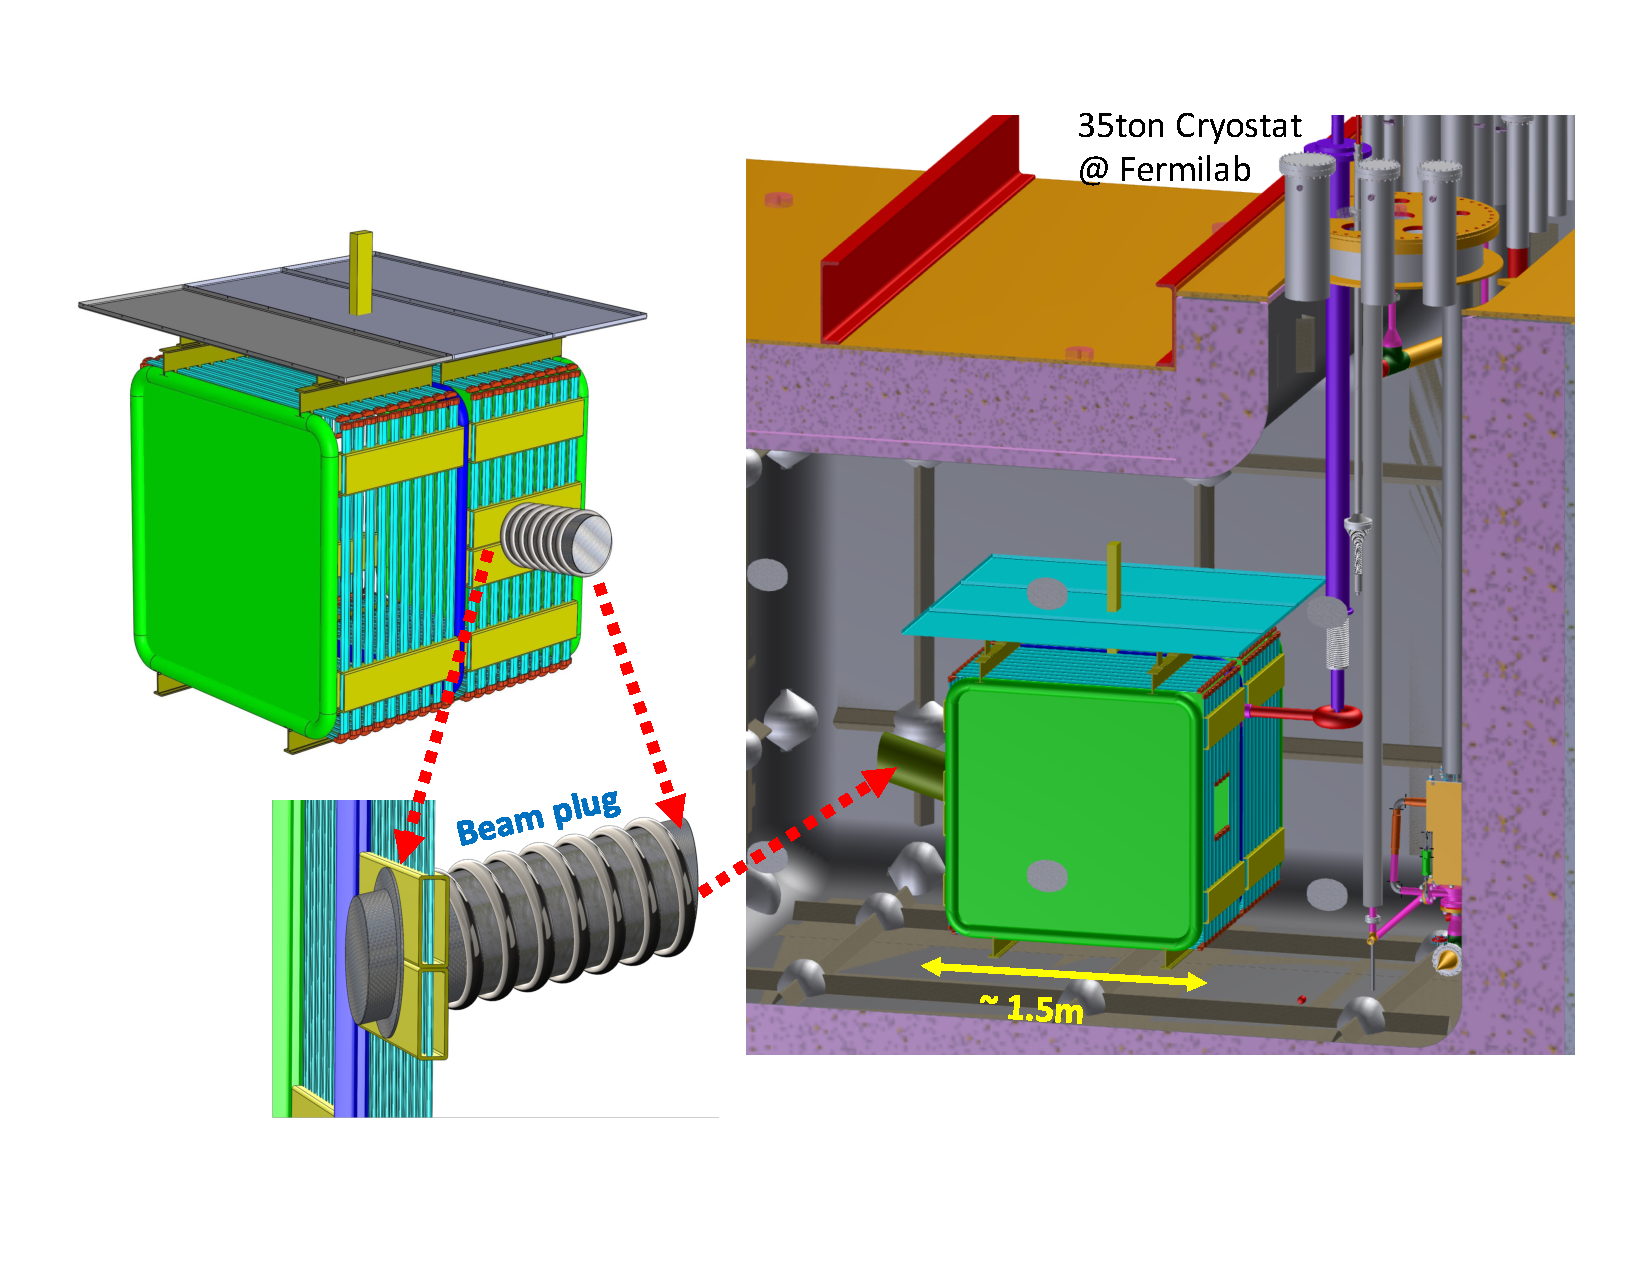
\includegraphics[width=0.95\textwidth]{beamwindow_PC4Test.pdf}
\end{cdrfigure}


%%%%%%%%%%%%%%%%%%%%%%%%%
\subsection{QC Procedures}


